  \subsection{Medición de potencia activa y factor de potencia} 
    Las conexiones explicadas se representan en el esquema de la Figura~\ref{fig:EsquemaConexiones}.
    Se hace uso de las atenuaciones que ofrece el osciloscopio digital, de forma tal que los valores
    que se miden sean exactamente los valores reales. Es decir, para el \textbf{canal 1}, en cual se mide
    la \textit{tensión de entrada} $\mathbf{V_i}$, se coloca una \textbf{atenuación x100} (x10 de la punta
    y x10 del divisor resistivo), y para el \textbf{canal 2}, en el cual se mide la \textit{corriente de entrada}
    $\mathbf{I_i}$ de forma indirecta por Ley de Ohm, se coloca una atenuación \textbf{atenuación x1}
    (debido a que $R\textsubscript{1}=10\ \Omega$).

    \begin{figure}[H]
      \centering
      \frame{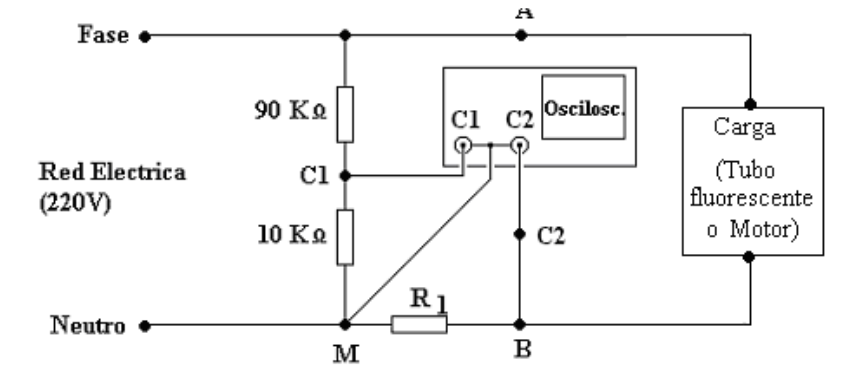
\includegraphics[width=0.7\textwidth]{Imagenes/ActividadPractica/EsquemaConexiones.png}}
      \caption{Esquema de conexiones para las mediciones.}
      \label{fig:EsquemaConexiones}
    \end{figure}

    \subsubsection{Medición de los módulos de tensión y corriente de entrada}
      En la Figura~\ref{fig:Vi_Ii} se puede ver los valores obtenidos al realizar la medición, los cuales
      se obtienen como valores \textit{root main square} (RMS), ya que se utilizan para el cálculo de 
      potencias. Las mediciones son:
      
      \begin{equation*}
        \boxed{V_{i_{RMS}} =  213 \ [V]} \hspace{20pt} ; \hspace{20pt} \boxed{I_{i_{RMS}} = 333\ [mA]}\ .
      \end{equation*}
      
      \begin{figure}[H]
        \centering
        \frame{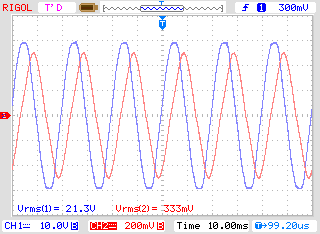
\includegraphics[width=0.4\textwidth]{Imagenes/ActividadPractica/MedicionDePotenciasYFdP/Exp1_1_Vin-Iin.png}}
        \caption{Medición de tensión y corriente de entrada con el osciloscopio.}
        \label{fig:Vi_Ii}
      \end{figure}
  
    \subsubsection{Medición de la diferencia de fase de la tensión y corriente de entrada}
    A continuación, se procede a calcular la \textbf{diferencia de fase} de la tensión y corriente de entrada.
    En la Figura~\ref{fig:DiferenciaDeFase} se aprecia la medición con el osciloscopio en modo dual y en modo X-Y.

    \begin{figure}[H]
      \centering
      \begin{subfigure}[h]{0.4\textwidth}
        \centering
        \frame{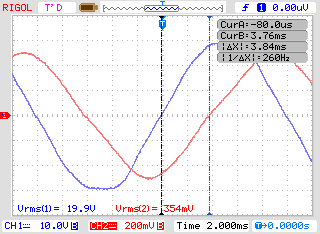
\includegraphics[width=\textwidth]{Imagenes/ActividadPractica/MedicionDePotenciasYFdP/Exp1_2_DiferenciaDeFaseEnSegundos.png}}
        \caption{Medición en modo dual.}
        \label{fig:DiferenciaDeFaseEnSegundos}
      \end{subfigure}
      \hspace{20pt} 
      \begin{subfigure}[h]{0.4\textwidth}
        \centering
        \frame{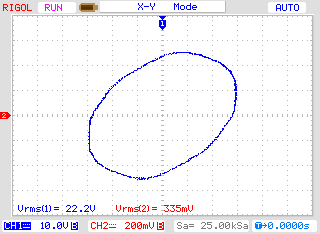
\includegraphics[width=\textwidth]{Imagenes/ActividadPractica/MedicionDePotenciasYFdP/Exp1_4_FiguraDeLissajous.png}}
        \caption{Medición en modo X-Y.}
        \label{fig:FiguraLissajous}
      \end{subfigure}
      \caption{Medición de diferencia de fase.}
      \label{fig:DiferenciaDeFase}
    \end{figure}

    \subsubsection*{Método 1: medición en modo dual}
    Simplemente, se procede a realizar una regla de tres simple, basándose en la Figura~\ref{fig:DesfaseEnSegundos}, mediante el
    semiperíodo de la tensión de entrada y la diferencia en segundos entre las señales. Por lo tanto, la diferencia de
    fase es

    \begin{align*}
      9,92\ ms &\longrightarrow 180\ ^{\circ} (semiperiodo) \\
      3,82\ ms &\longrightarrow \varphi = \dfrac{3,84\ ms \cdot 180\ ^{\circ}}{9,92\ ms} \hspace{20pt} \Longrightarrow \hspace{20pt} \Aboxed{\varphi=69,67\ ^{\circ}}\ .
    \end{align*}

    \begin{figure}[H]
      \centering
      \begin{subfigure}[h]{0.4\textwidth}
        \centering
        \frame{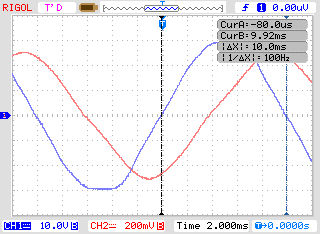
\includegraphics[width=\textwidth]{Imagenes/ActividadPractica/MedicionDePotenciasYFdP/Exp1_9_SemiperiodoEnSegundos.png}}
        \caption{Semiperíodo en segundos.}
        \label{fig:SemiperiodoEnSegundos}
      \end{subfigure}
      \hspace{20pt} 
      \begin{subfigure}[h]{0.4\textwidth}
        \centering
        \frame{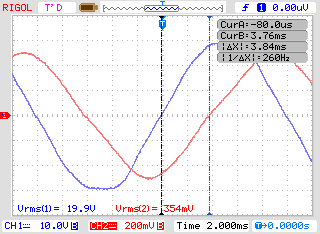
\includegraphics[width=\textwidth]{Imagenes/ActividadPractica/MedicionDePotenciasYFdP/Exp1_2_DiferenciaDeFaseEnSegundos.png}}
        \caption{Desfase de las señales en seg.}
        \label{fig:DiferenciaDetiempoDeLasSeñales}
      \end{subfigure}
      \caption{Medición de diferencia de fase en modo dual.}
      \label{fig:DesfaseEnSegundos}
    \end{figure}

    \subsubsection*{Método 2: medición en modo X-Y}
    Este método se basa en el uso de la figura de Lissajous mostrada en el osciloscopio. Las mediciones se pueden ver en la 
    Figura~\ref{fig:DesfaseConLissajous}. En base a la ecuación~(\ref{eqn:AngDeDesf}) se calcula el valor de la 
    \textbf{diferencia de fase}
    
    \begin{align*}
      \varphi = sen ^{-1} \left( \dfrac{A}{B} \right) = sen ^{-1} \left( \dfrac{0,944\ V}{1,01\ V} \right) \hspace{20pt} \Longrightarrow \hspace{20pt} \Aboxed{\varphi = 69,17\ ^{\circ}}\ .
    \end{align*}

    \begin{figure}[H]
      \centering
      \begin{subfigure}[h]{0.4\textwidth}
        \centering
        \frame{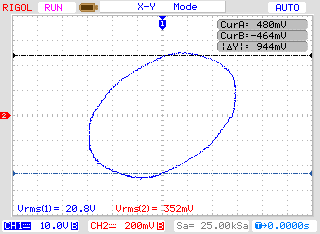
\includegraphics[width=\textwidth]{Imagenes/ActividadPractica/MedicionDePotenciasYFdP/Exp1_6_CortesEjeYFigLis.png}}
        \caption{Valores de corte de la figura en el eje vertical (A).}
        \label{fig:CortesEjeVertical_Lissajous}
      \end{subfigure}
      \hspace{20pt} 
      \begin{subfigure}[h]{0.4\textwidth}
        \centering
        \frame{\includegraphics[width=\textwidth]{Imagenes/ActividadPractica/MedicionDePotenciasYFdP/Exp1_7_MáximosEjeVertical.png}}
        \caption{Valores máximos de la figura en el eje vertical (B).}
        \label{fig:MaximosEjeVertical_Lissajous}
      \end{subfigure}
      \caption{Medición de diferencia de fase en  modo X-Y.}
      \label{fig:DesfaseConLissajous}
    \end{figure}


    Con las mediciones anteriores ya realizadas, se calculan las potencias \textbf{activa} (P), \textbf{reactiva} (Q)
    y \textbf{aparente} (S), con el uso de las ecuaciones~(\ref{eqn:PotActTot}), (\ref{eqn:PotReacTot}) y 
    (\ref{eqn:PotApaTot}) respectivamente

    \begin{align*}
      P &= V_i  I_i  \cos(\varphi) = 213\ V \cdot 0,333\ A \cdot \cos(69,17\ ^{\circ}) 
                                \hspace{20pt} \therefore \hspace{20pt} \Aboxed{P = 25,22\ [W]} \\
      Q &= V_i  I_i  \sen(\varphi) = 213\ V \cdot 0,333\ A \cdot \sin(69,17\ ^{\circ}) 
                                \hspace{20pt} \therefore \hspace{20pt} \Aboxed{Q = 66,29\ [VAR]} \\
      S &= \sqrt{P^2 + Q^2} =  \sqrt{(25,22\ W)^2 + (66,29\ VAR)^2}
                                \hspace{20pt} \therefore \hspace{20pt} \Aboxed{S = 70,92\ [VA]} \ .
    \end{align*}

    \noindent De la misma forma, con la ecuación~(\ref{eqn:fpFinal}) se calcula el factor de potencia \textbf{fp}
    \begin{align*}
      fp = cos(\varphi) = cos(69,17 ^{\circ}) \hspace{20pt} \therefore \hspace{20pt} \Aboxed{fp = 0,36}\ .
    \end{align*}



